\subsection{Simulação 1 - Extremidades da pá}

É fácil observar que as áreas de mais difícil acesso à pá são suas extremidades,
áreas em preto da figura~\ref{fig::extremidades}, devido ao alcance do robô e
por serem áreas em que a pá apresenta maior inclinação, o que afeta bastante na
direção dos vetores normais à pá. A alteração da direção da normal e a posição
do ponto a ser revestido são os fatores mais importantes para o aplicação de
revestimento, logo pontos em uma posição elevada para o robô e normal
direcionada para cima são complexos. Observe a figura~\ref{fig::normal}, o vetor
$\vec{P}$ é um exemplo de vetor normal pertencente a um ponto da pá de difícil
revestimento, tanto pela posição quanto pelo vetor normal.

\begin{figure}[!ht]
	\centering	
	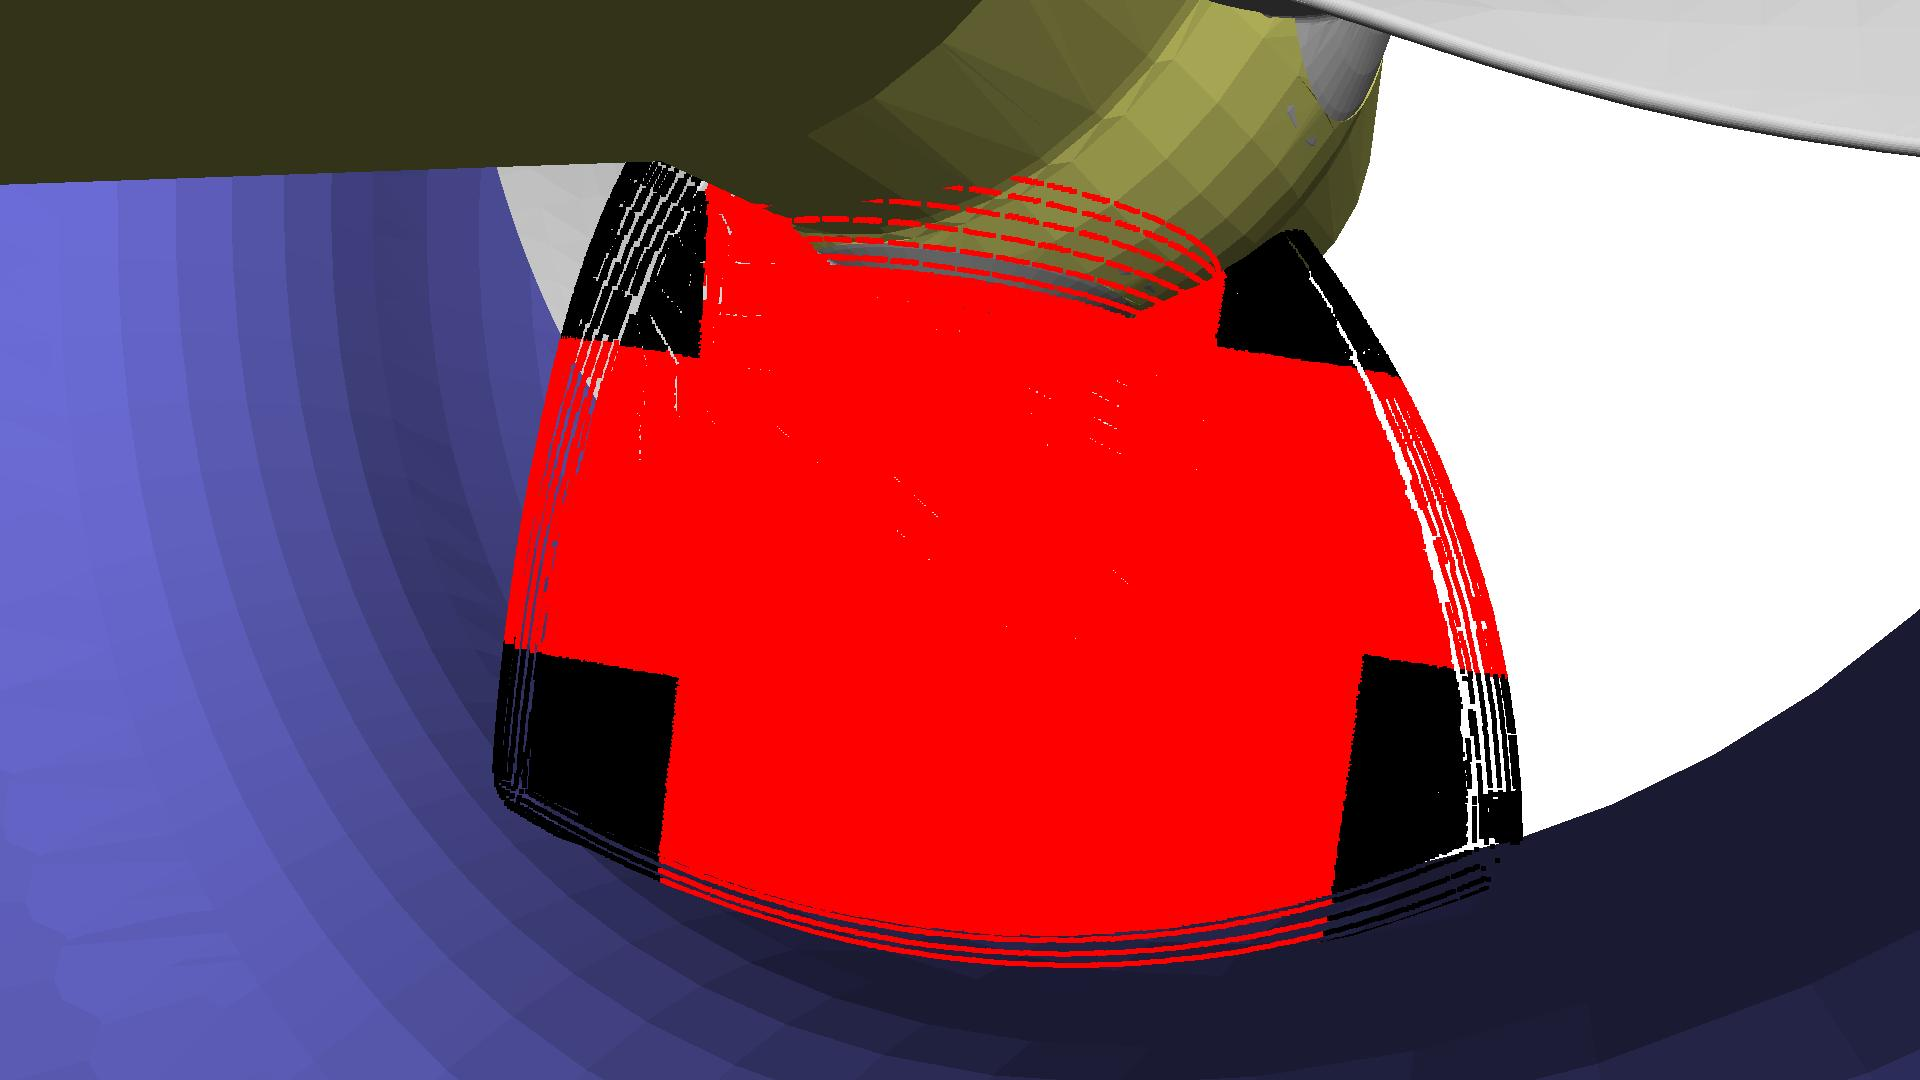
\includegraphics[width=.8\columnwidth]{figs/tocoat.jpg}
	\caption{Extremidades da pá em preto.}
	\label{fig::extremidades}
\end{figure}

\begin{figure}[!ht]
	\centering	
	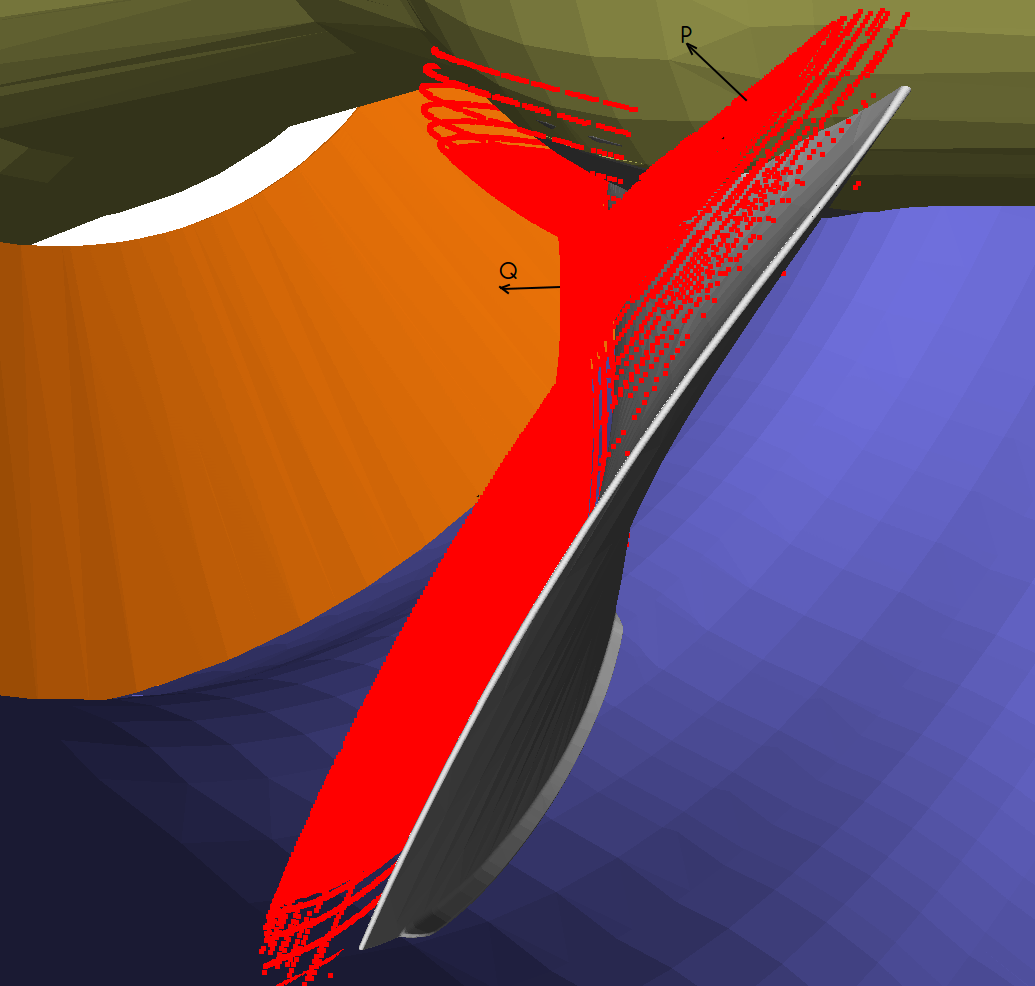
\includegraphics[width=.5\columnwidth]{figs/normal.png}
	\caption{Vetores normais (em preto) de pontos a serem revestidos (em
	vermelho).}
	\label{fig::normal}
\end{figure}

A simulação de teste de revestimento das extremidades considerou as seguintes
variáveis: 

\begin{itemize}
  \item O ângulo das pás da turbina foram fixados em $24^o$, ângulo natural de
  uso.
  \item O rotor da turbina foi girado de $0^o$ a $30^o$ com passo de $3^o$.
  \item A distância entre extremidade da pistola e pá pode variar $235
  \pm 5$ mm.
  \item O ângulo entre a pistola e o plano da pá pode variar $90^o \pm
  30^o$.
  \item A posição em $y$ do robô pode variar $-2970 \pm 250$ mm (posição
  global) com passo de 50 mm.
  \item A posição em $x$ do robô pode variar $980 \pm 750$ mm em relação à pá
  com passo de 50 mm.
  \item A posição em $z$ do robô foi amostrada uniformemente em 7 pontos ao
  longo da pá.
\end{itemize}

A figura~\ref{fig::trilho2all} mostra todas as posições simuladas para a base do
robô. As restrições dessas posições são a altura mínima da base ao aro câmara e
a altura do robô. Para cada posição de base e ângulo do rotor, foi simulado o
processo de revestimento para as quatro extremidades da pá, levando em
consideração as tolerâncias.

\begin{figure}[!ht]
	\centering	
	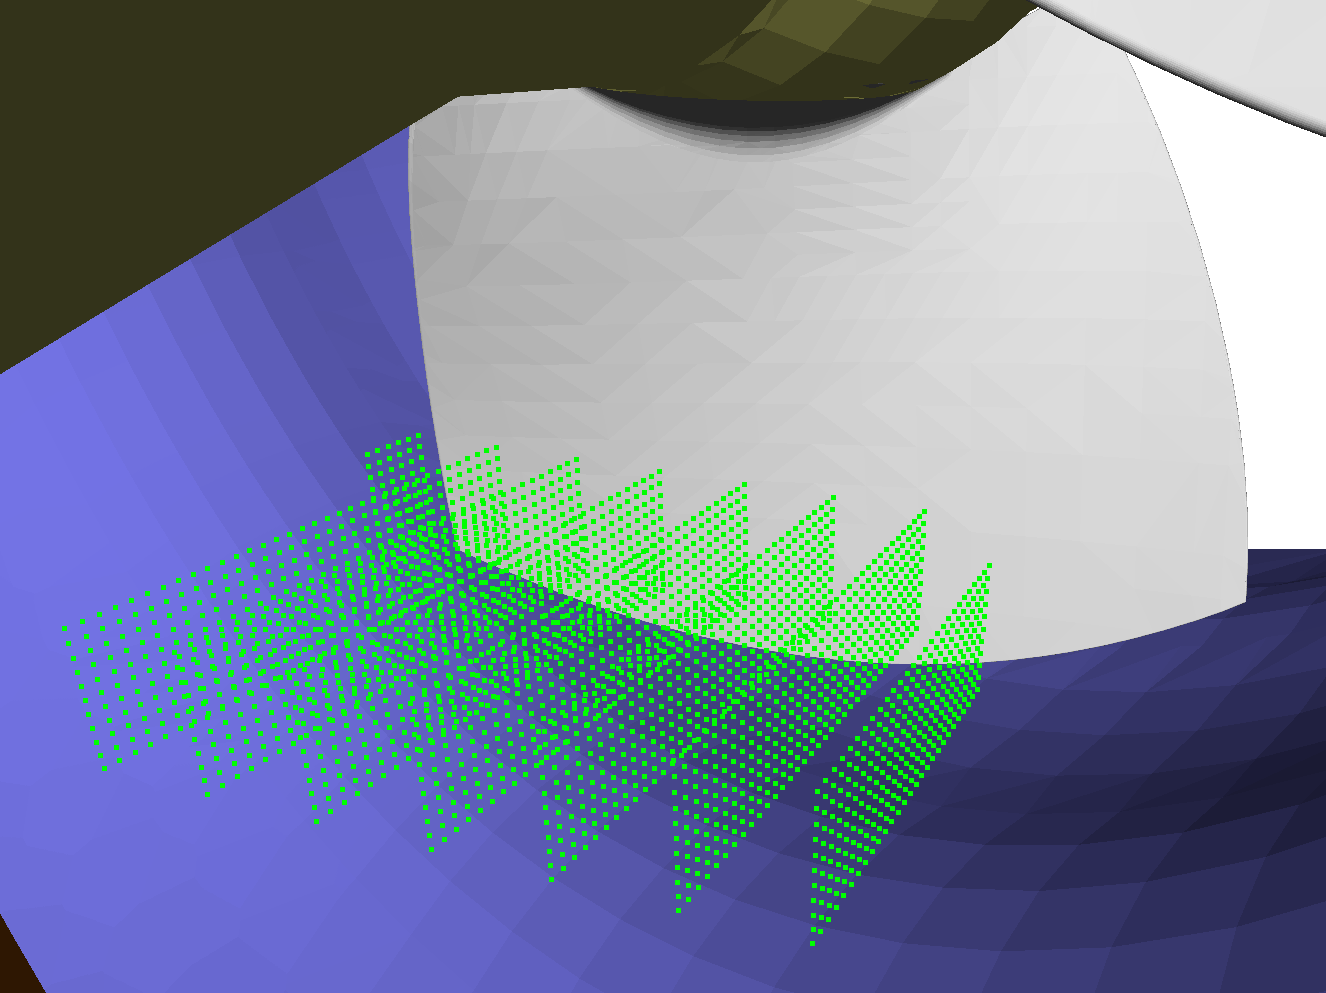
\includegraphics[width=1\columnwidth]{figs/trilho2all.png}
	\caption{Possíveis posições da base do robô, em verde.}
	\label{fig::trilho2all}
\end{figure}

Nas subseções seguintes, serão analisadas cada extremidade da
pá independentemente, considerando as varíaveis acima.

\subsubsection{Extremidade inferior esquerda}

A extremidade inferior esquerda apresenta a complexidade de posição do ponto a
ser revestido, visto que os pontos estão na borda, próximas ao aro câmara,
aumentando o risco de colisões. A figura~\ref{fig::footleft} mostra a
discretização da pá na extremidade esquerda: pontos azuis são pontos revestidos
na tolerância de $30^o$; em preto, pontos revestidos sem tolerância; e em
vermelho, pontos que não foram revestidos para esta posição do robô.

\begin{figure}[!ht]
	\centering	
	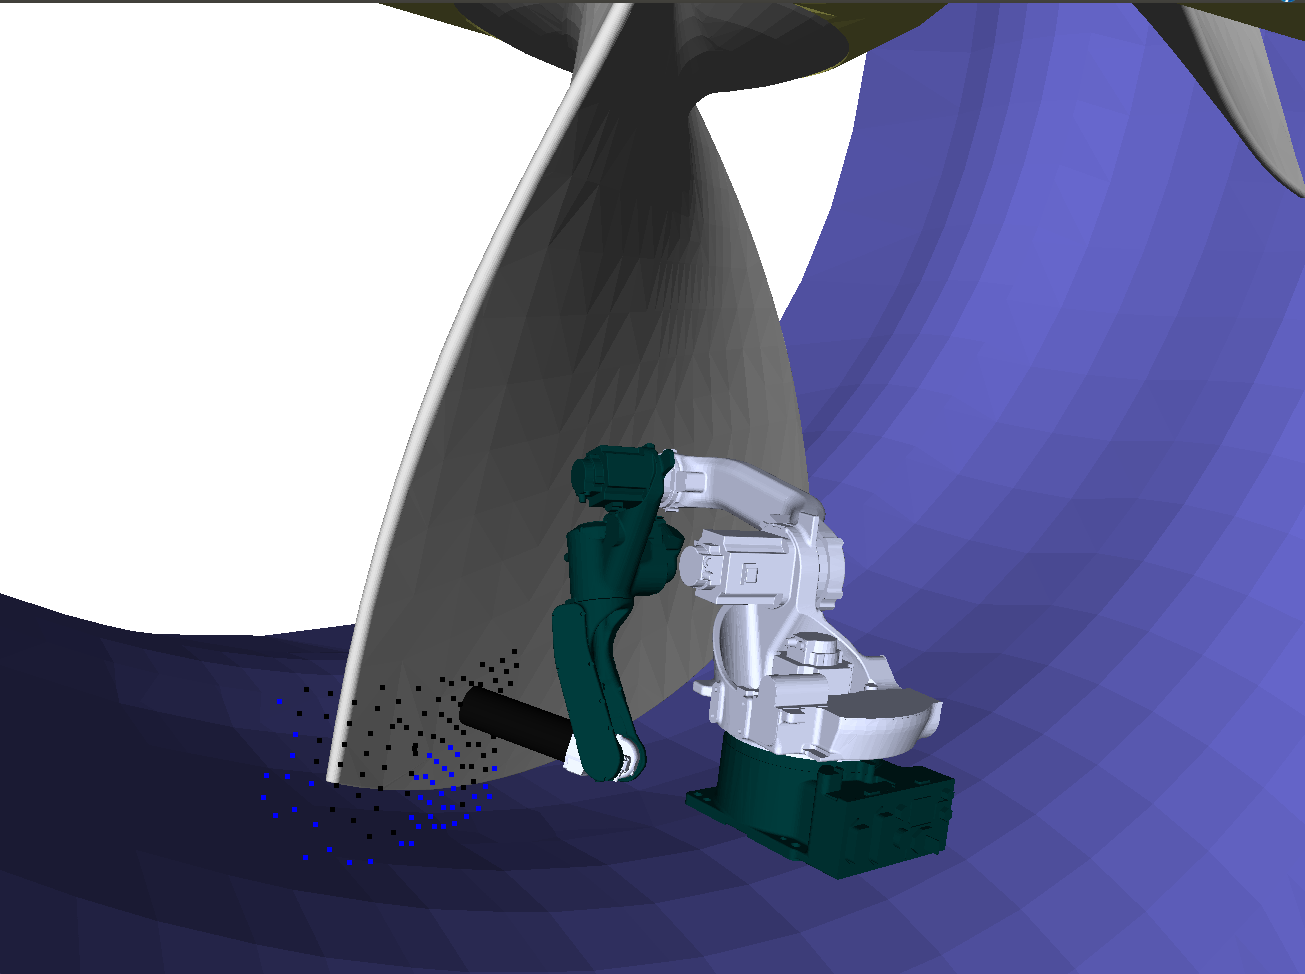
\includegraphics[width=1\columnwidth]{figs/footleft.png}
	\caption{Estudo de revestimento para a extremidade inferior esquerda.}
	\label{fig::footleft}
\end{figure}

A simulação mostrou que o robô foi capaz de revestir toda a extremidade, na
altura mínima $y=-3220$ mm, a uma distância de até $x=1300$ mm da pá. Conforme o
robô se aproxima da pá, verifica-se que a altura pode sofrer variações
positivas, por exemplo para $x=980$ mm, $y=-3070$ mm. Entretanto, como já foi
verificado na simulação dinâmica, não é aconselhável aproxima o robô da pá a uma
distância inferior a $x=1000$ mm, pois os torques durante a execução podem ser
elevados.

Dessa forma, a extremidade inferior esquerda não mostrou desafios técnicos.

\subsubsection{Extremidade inferior direita}

A extremidade inferior direita possui complexidade de posição do ponto a
ser revestido maior que a extremidade inferior esquera, visto que a extremidade
está mais próxima da área em que a curvatura do aro é superior a $20^o$ (base
mais próxima do solo). A figura~\ref{fig::footright} mostra a discretização da
pá na extremidade esquerda: pontos azuis são pontos revestidos na tolerância de
$30^o$; em preto, pontos revestidos sem tolerância; e em vermelho, pontos que
não foram revestidos para esta posição do robô.

\begin{figure}[!ht]
	\centering	
	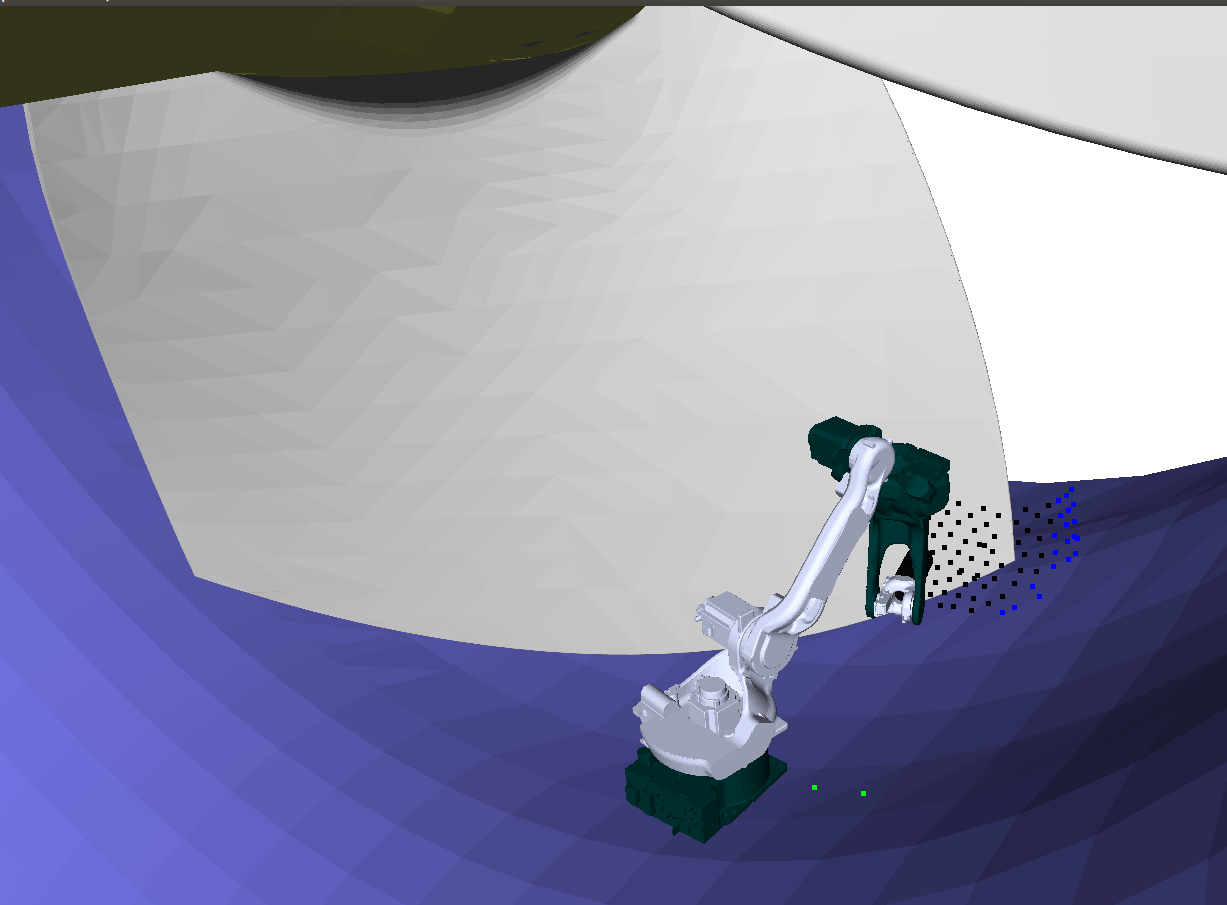
\includegraphics[width=1\columnwidth]{figs/footright.png}
	\caption{Estudo de revestimento para a extremidade inferior direita.}
	\label{fig::footright}
\end{figure}

A simulação mostrou que o robô foi capaz de revestir toda a extremidade, na
altura mínima $y=-3220$ mm, a uma distância de até $x=1300$ mm da pá. 

Dessa forma, a extremidade inferior direita não mostrou desafios técnicos.

\subsubsection{Extremidade superior esquerda}

A extremidade superior esquerda possui complexidade de posição do ponto a
ser revestido devido à altura do robô. A figura~\ref{fig::shoulderleft} mostra
a discretização da pá na extremidade esquerda: pontos azuis são pontos revestidos na tolerância de
$30^o$; em preto, pontos revestidos sem tolerância; e em vermelho, pontos que
não foram revestidos para esta posição do robô.

\begin{figure}[!ht]
	\centering	
	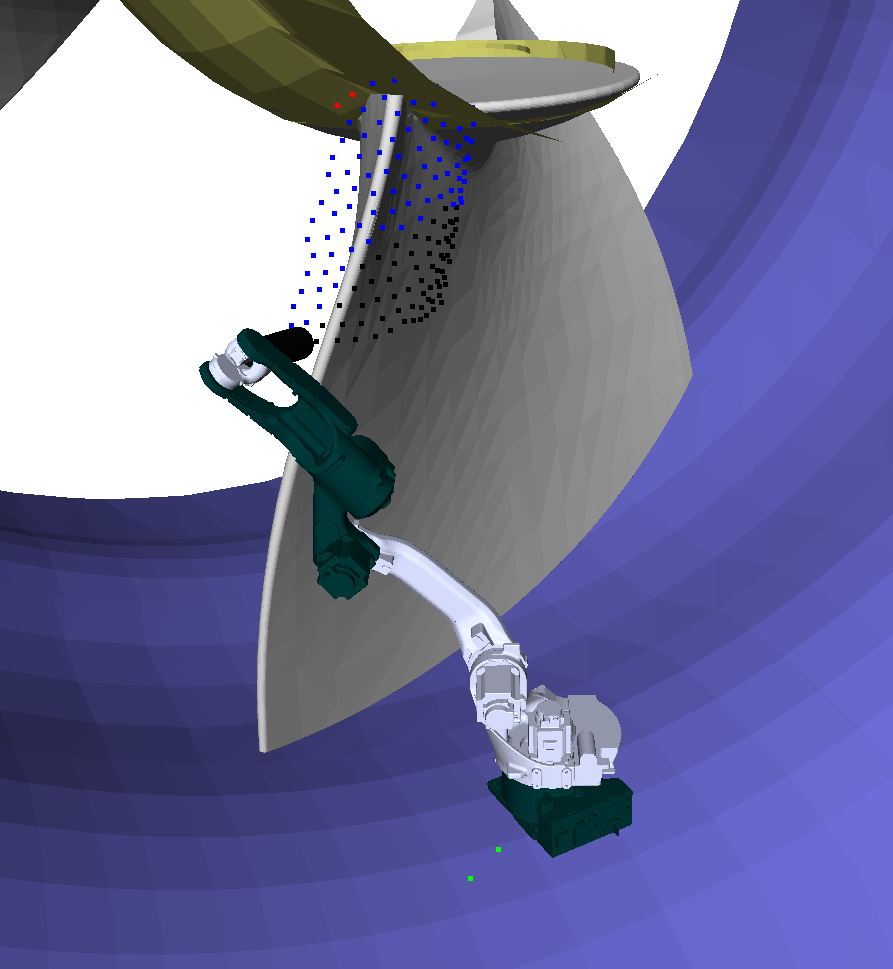
\includegraphics[width=1\columnwidth]{figs/shoulderleft.png}
	\caption{Estudo de revestimento para a extremidade superior esquerda.}
	\label{fig::shoulderleft}
\end{figure}

A simulação mostrou que se mantivermos a altura da base em $y=-3220$ mm
(altura mínima) e $x=1300$ mm, são necessárias duas posições em $z$ (ao longo do
trilho) para o revestimento completo da extremidade. É interessante para o
projeto manter altura fixa o quanto possível, pois há redução de grau de
liberdade, e, portanto, redução na complexidade da base mecânica.

Caso haja alteração na altura do robô, por exemplo  $y=-2770$ mm, só será
necessária uma posição em $z$ para a conertura completa da região. Mas é
preferível mover o robô no trilho, em $z$, a mover o robô em altura, em $y$. 

A extremidade superior esquerda necessitou duas posições para a base, mas não
mostrou desafios técnicos.

\subsubsection{Extremidade superior direita}

A extremidade superior esquerda possui duas complexidades de revestimento:
posição do ponto devido à altura do robô; e vetor normal, direção de
revestimento. A figura~\ref{fig::shoulderright} mostra a discretização da pá na
extremidade esquerda: pontos azuis são pontos revestidos na tolerância de $30^o$; em preto, pontos revestidos sem tolerância; e em vermelho, pontos que
não foram revestidos para esta posição do robô.

\begin{figure}[!ht]
	\centering	
	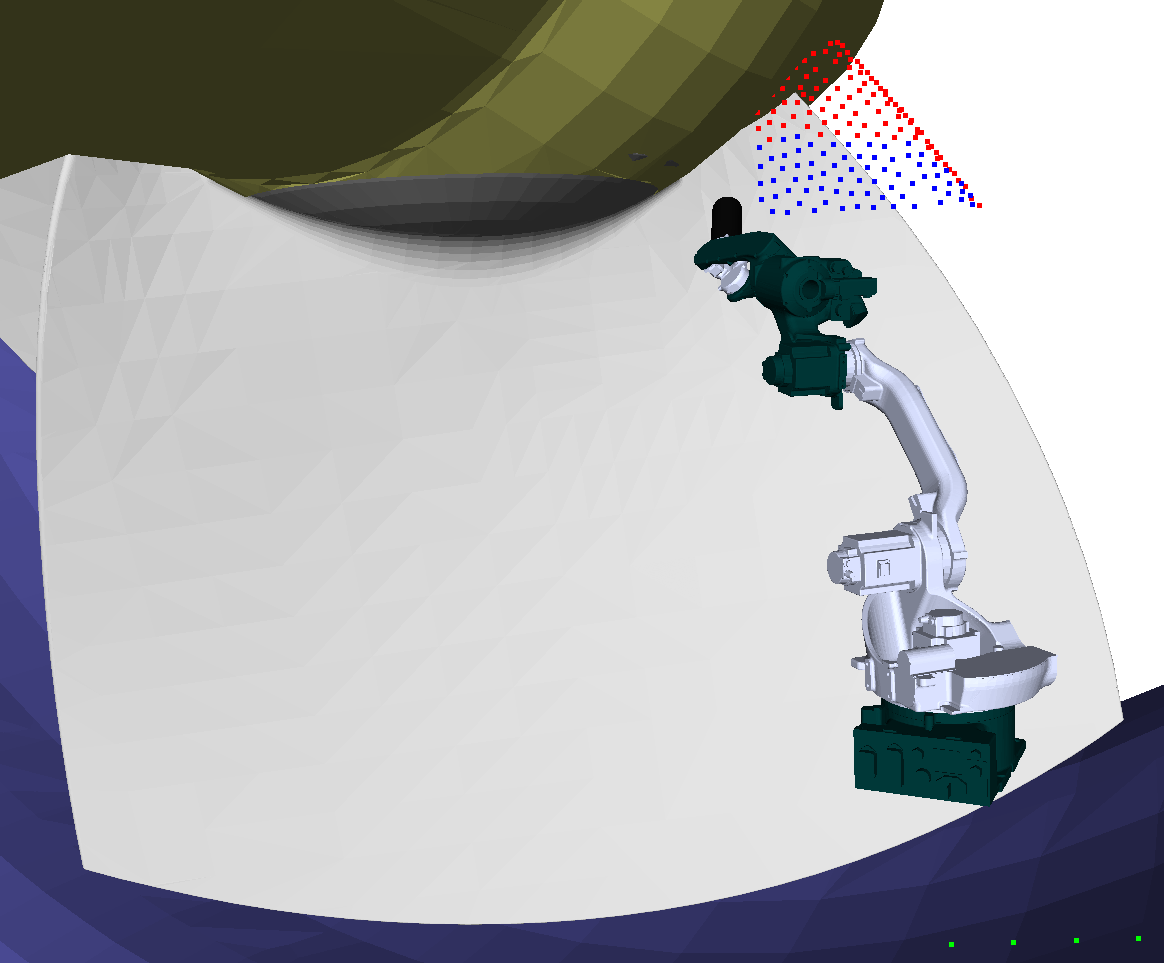
\includegraphics[width=1\columnwidth]{figs/shoulderright.png}
	\caption{Estudo de revestimento para a extremidade superior direita.}
	\label{fig::shoulderright}
\end{figure}

A simulação mostra que, mesmo se utilizarmos a altura máxima para a base
$y=-2720$ mm e mantivermos $x=1300$ mm, não há posição em $z$ (ao longo do
trilho) para revestir por completo a extremidade. Aproximando o manipulador da
pá, novos pontos são revestido, mas mesmo em $x=230$ mm o
revestimento não é completo. O mesmo teste foi feito para diferentes
ângulos do rotor, mas os resultados não são favoráveis, pois conforme o rotor
gira, a pá se afasta do robô.

Para $y=-3220$ mm e $x=1300$ mm, nenhum ponto da extremidade superior direita é
revestido, logo outras estratégias devem ser adotadas. A extremidade superior
direita mostrou grande complexidade técnica e não foi possível encontrar uma
solução viável para o 2º trilho a fim de revestí-la.